\documentclass[main.tex]{subfiles}
\begin{document}
\begin{enumerate}

\subsection*{Section 6: Electronics, Photonics \& MEMS}

\item [16.] Provide clear explanations to the following questions:

    \begin{enumerate}
        \item \textbf{Q.} Using band-theory and energy-related arguments, explain why a metal conducts, an insulator blocks current, and a semiconductor conducts current only under certain situations. \textbf{A.} In metals, the valence band and conduction band overlap, allowing electrons to move freely through the material and conduct electricity. In insulators, the valence band is completely filled with electrons and the conduction band is empty or separated by a large energy gap. This makes it difficult for electrons to move from the valence band to the conduction band and thus blocks current. In semiconductors, the valence band is completely filled with electrons while the conduction band is empty or separated by a small energy gap. This allows electrons to move from the valence band to the conduction band when excited by thermal energy or other means, thus allowing current to flow through the material. Depending on the material and the degree of detail desired, a variety of energy levels will be plotted against position:
        
        \begin{itemize}
            \item $E_{\mathrm{F}}$ or $\mu$ : Although it is not a band quantity, the Fermi level (total chemical potential of electrons) is a crucial level in the band diagram. The Fermi level is set by the device's electrodes. For a device at equilibrium, the Fermi level is a constant and thus will be shown in the band diagram as a flat line. Out of equilibrium (e.g., when voltage differences are applied), the Fermi level will not be flat. Furthermore, in semiconductors out of equilibrium it may be necessary to indicate multiple quasi-Fermi levels for different energy bands, whereas in an out-of-equilibrium insulator or vacuum it may not be possible to give a quasi-equilibrium description, and no Fermi level can be defined.
            \item $E_{\mathrm{C}}$ : The conduction band edge should be indicated in situations where electrons might be transported at the bottom of the conduction band, such as in an $n$-type semiconductor. The conduction band edge may also be indicated in an insulator, simply to demonstrate band bending effects.
            \item $E_{\mathrm{V}}$ : The valence band edge likewise should be indicated in situations where electrons (or holes) are transported through the top of the valence band such as in a p-type semiconductor.
            \item $E_{\mathrm{i}}$ : The intrinsic Fermi level may be included in a semiconductor, to show where the Fermi level would have to be for the material to be neutrally doped (i.e., an equal number of mobile electrons and holes).
            \item $E_{\text {imp }}$ : Impurity energy level. Many defects and dopants add states inside the band gap of a semiconductor or insulator. It can be useful to plot their energy level to see whether they are ionized or not.
            \item $E_{\mathrm{vac}}$ : In a vacuum, the vacuum level shows the energy $-e \phi$, where $\phi$ is the electrostatic potential. The vacuum can be considered as a sort of insulator, with $E_{\mathrm{vac}}$ playing the role of the conduction band edge. At a vacuum-material interface, the vacuum energy level is fixed by the sum of work function and Fermi level of the material.
            \item Electron affinity level: Occasionally, a "vacuum level" is plotted even inside materials, at a fixed height above the conduction band, determined by the electron affinity. This "vacuum level" does not correspond to any actual energy band and is poorly defined (electron affinity strictly speaking is a surface, not bulk, property); however, it may be a helpful guide in the use of approximations such as Anderson's rule or the Schottky-Mott rule.
        \end{itemize}

        \begin{figure}
        \centering\fbox{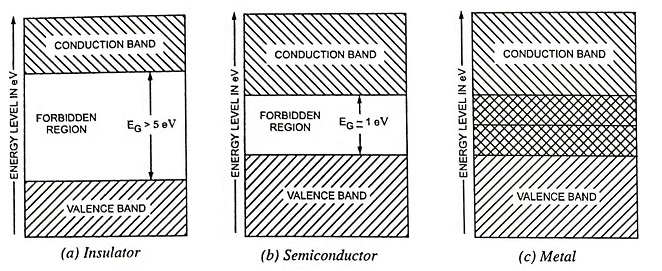
\includegraphics[width=3.0in]{2018spring/figures/16a_a.png}}
        \caption{Band theory of insulator, semiconductor, and metal}
        \label{fig:17q_a}
        \end{figure}
        
        \item \textbf{Q.} A PN junction is used as a photodetector. Assume that light is shining on all parts of the diode equally. Which part of the photodiode is most critical for photo detection and why? In this application, should the devices be under forward or reverse bias? 
        
        \textbf{A.} Forward biasing means putting a voltage across a diode that allows current to flow easily, while reverse biasing means putting a voltage across a diode in the opposite direction. A photodiode is a semiconductor device with a P-N junction that converts photons (or light) into electrical current. The P layer has an abundance of holes (positive), and the N layer has an abundance of electrons (negative). Photodiodes can be manufactured from a variety of materials including, but not limited to, Silicon, Germanium, and Indium Gallium Arsenide. Each material uses different properties for cost benefits, increased sensitivity, wavelength range, low noise levels, or even response speed. 

        \begin{figure}
        \centering\fbox{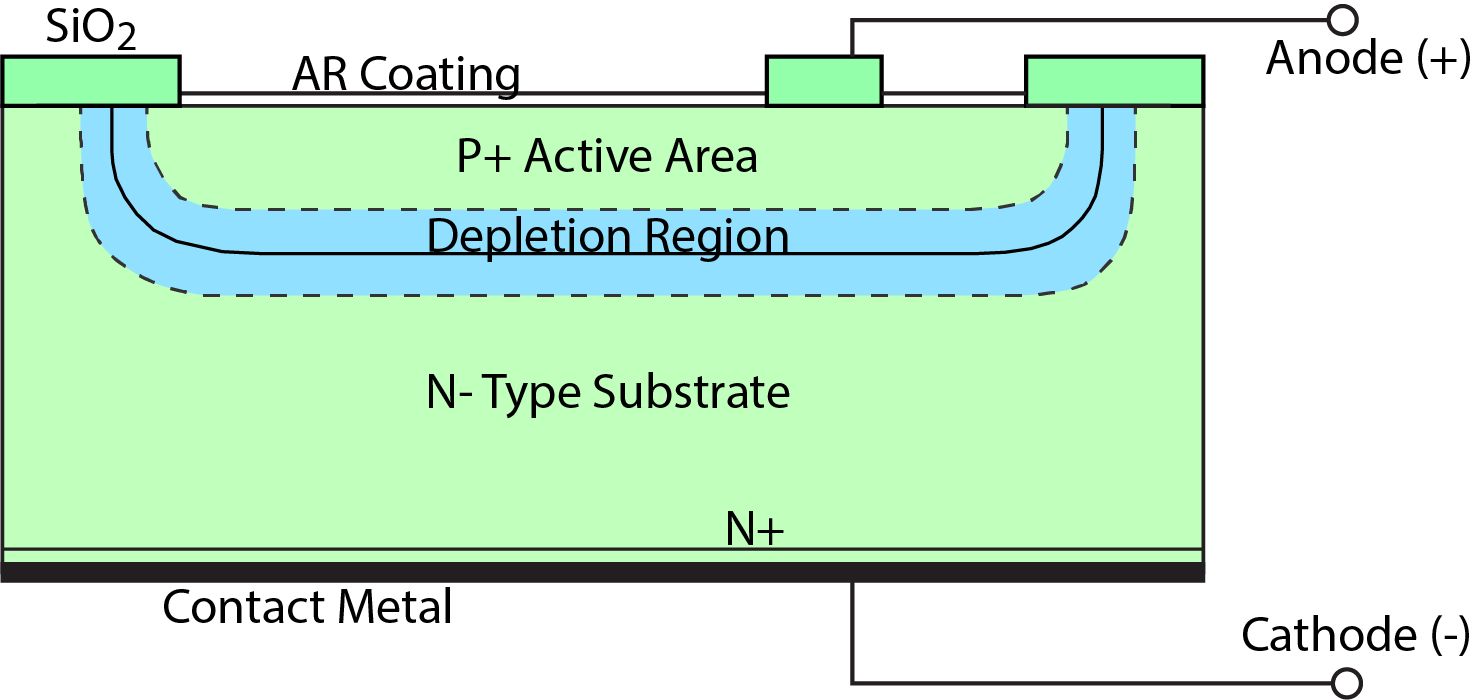
\includegraphics[width=4.0in]{2018spring/figures/16a_b.png}}
        \caption{P-N Photodiode Cross-section}
        \label{fig:16a_b}
        \end{figure}
        
        Figure \ref{fig:16a_b} shows a cross section of a typical photodiode. A \textbf{Depletion Region} is formed from diffusion of electrons from the N layer to the P layer and the diffusion of holes from the P layer to the N layer. This creates a region between the two layers where no free carriers exist. This develops a built-in voltage to create an electric field across the depletion region. This allows for current to flow only in one direction (Anode to Cathode). The photodiode can be forward biased, but current generated will flow in the opposite direction. This is why most photodiodes are reversed biased or not biased at all. Some photodiodes cannot be forward biased without damage.

        A photon can strike an atom within the device and release an electron if the photon has enough energy. This creates an electron-hole pair (e- and h+) where a hole is simply an “empty space” for an electron. If photons are absorbed in either the P or N layers, the electron hole pairs will be recombined in the materials as heat if they are far enough away (at least one diffusion length) from the depletion region. Photons absorbed in the depletion region (or close to it) will create electron hole pairs that will move to opposite ends due to the electric field. Electrons will move toward the positive potential on the Cathode, and the holes will move toward the negative potential on the Anode. These moving charge carriers form the current (photocurrent) in the photodiode. Figure \ref{fig:16a_b} shows the different layers of a photodiode (P-N Junction) as well as multiple connection points on top and bottom. The depletion region creates a capacitance in the photodiode where the boundaries of the region act as the plates of a parallel plate capacitor. Capacitance is inversely proportional to the width of the depletion region. Reverse bias voltage also influences the capacitance of the region. There are four major parameters used in choosing the right photodiode and whether or not to reverse bias the photodiode.

        \begin{itemize}
            \item Response (speed/time) of the photodiode is determined by the capacitance of the P-N junction. It is the time needed for charge carriers to cross the P-N junction. This is directly affected by the width of the depletion region.
            \item Responsivity is the ratio of photocurrent generated from incident light, to that incident light power. This is usually expressed in units of A/W (current over power). A typical responsivity curve of a photodiode will show A/W as a function of wavelength. This is called Quantum Efficiency.
            \item Dark current is the current in the photodiode when there is no incident light. This can be one of the main sources of noise in the photodiode system. Photocurrent from background radiation can also be included in this measurement. Photodiodes are usually put into an enclosure that does not allow any light to hit the photodiode to measure the dark current. Because the current generated by the photodiode can be very small, dark current levels can obscure the current produced by incident light at low light levels. Dark current increases with temperature. Without biasing, the dark current can be very low. The ideal photodiode would have no dark current.
            \item Breakdown Voltage is the largest reverse voltage that can be applied to the photodiode before there is an exponential increase in leakage current or dark current. Photodiodes should be operated below this maximum applied reverse bias or damage to the photodiode may occur. Breakdown voltage decreases with an increase in temperature.
        \end{itemize}

        \begin{figure}
        \centering\fbox{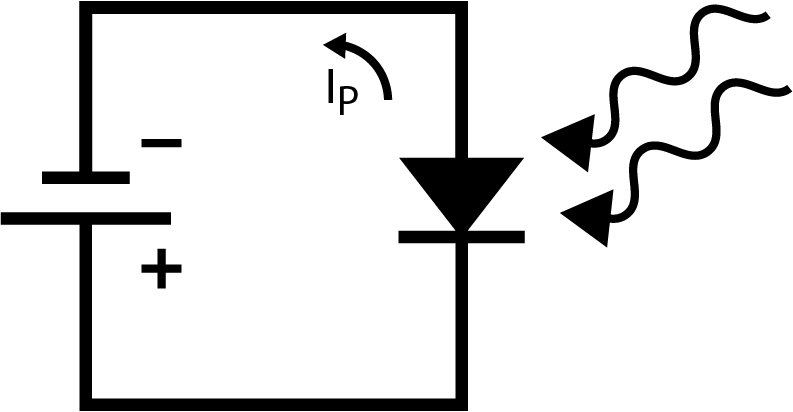
\includegraphics[width=3.0in]{2018spring/figures/16a_c.png}}
        \caption{PHOTOCONDUCTIVE MODE REVERSE BIASED}
        \label{fig:16a_c}
        \end{figure}

        When the photodiode is reverse biased (Figure \ref{fig:16a_c}), an external voltage is applied to the P-N junction. The negative terminal is connected to the positive P layer, and the positive terminal is connected to the negative N layer. This causes the free electrons in the N layer to pull toward the positive terminal, and the holes in the P layer to pull toward the negative terminal. When the external voltage is applied to the photodiode, the free electrons start at the negative terminal and immediately fill the holes in the P layer with electrons. This creates negative ions in the atoms with extra electrons. The charged atoms then oppose the flow of free electrons to the P layer. Similarly, holes go about the same process to create positive ions but in the opposite direction. When reverse biased, current will only flow through the photodiode with incident light creating photocurrent. The reverse bias causes the potential across the depletion region to increase and the width of the depletion region to increase. This is ideal for creating a large area to absorb the maximum amount of photons. The response time is reduced by the reverse bias by increasing the size of the depletion layer. This increased width reduces the junction capacity and increases the drift velocity of the carriers in the photodiode. The transit time of the carriers is reduced, improving the response time. Unfortunately, increasing the bias current increases the dark current as well. This noise can be a problem for very sensitive systems using P-N or PIN photodiodes. This hinders the performance in low light situations. If using APDs, the signal to noise ratio will be large regardless because of the gain of the photodiode. Because a photon is ideally absorbed in the depletion region, the P layer can be constructed to be extremely thin. This can be balanced with the reverse bias to create an optimal photodiode with a faster response time while maintaining as low as noise as possible.
        
        \item \textbf{Q.} After repeated operations of a PMOS MOSFET, hole-type interface traps are formed in the Si-SiO2 interface, does this process increase or decrease the threshold voltage? Draw the band-diagram and the sub-threshold IV curve to illustrate your answer. \textbf{Theory.} The threshold voltage, commonly abbreviated as $\mathrm{V}_{\mathrm{th}}$ or $\mathrm{V}_{\mathrm{GS}(\mathrm{th})}$, of a field-effect transistor (FET) is the minimum gate-to-source voltage $\left(V_{G S}\right)$ that is needed to create a conducting path between the source and drain terminals. It is an important scaling factor to maintain power efficiency. In semiconductor production, doping is the intentional introduction of impurities into an intrinsic semiconductor for the purpose of modulating its electrical, optical and structural properties. The construction and working of a PMOS is same as NMOS. A lightly doped n-substrate is taken into which two heavily doped P+ regions are diffused. These two P+ regions act as source and drain. A thin layer of SiO2 is grown over the surface. Holes are cut through this layer to make contacts with P+ regions, as shown in the figure \ref{fig:16a_d}.

        \begin{figure}
        \centering\fbox{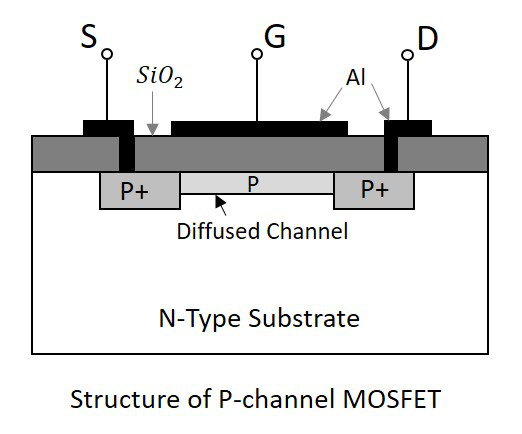
\includegraphics[width=3.0in]{2018spring/figures/16a_d.png}}
        \caption{PMOS (P-channel) MOSFET}
        \label{fig:16a_d}
        \end{figure}

        \textbf{A.} The band diagram is shown in Figure \ref{fig:16a_e} and the sub-threshold IV curve is shown in figure \ref{fig:16a_f}. Negative Bias Temperature Instability (NBTI) is an increase in the absolute threshold voltage, a degradation of the mobility, drain current, and transconductance of p-channel MOSFETs. These typesof effects are generally found in pMOSFETs. When a PMOS transistor is biased in inversion, the dissociation of $\mathrm{Si}-\mathrm{H}$ bonds along the silicon-oxide interface causes the generation of interface traps. The rate of generation of these traps is accelerated by temperature, and the time of applied stress. These traps cause an increase in the threshold voltage $\left(\mathrm{V}_{\mathrm{th}}\right)$ of the PMOS transistors. An increase in $\mathrm{V}_{\mathrm{th}}$ causes the circuit delay to degrade, and when this degradation exceeds a certain magnitude, the circuit may fail to meet its timing specifications. This effect is known as the Negative Bias Temperature Instability (NBTI). Mechanism of NBTI is the degradation of $\mathrm{Si}-\mathrm{H}$ bonds broken by the chemical reaction with high energy holes on $\mathrm{SiO}_2 / \mathrm{Si}$ surface. In PMOS voltage between gate and the source is negative $\left(\mathrm{V}_{\mathrm{gs}}=-\mathrm{V}_{\mathrm{du}}\right)$, causes the interface traps and when $\left(\mathrm{V}_{\mathrm{gs}}=0\right)$ causes the reduction in the interface traps. Thus the effect of NBTI on the PMOS depends on the time the device has been stressed, and relaxed. It is commonly accepted that two kinds of trap contribute to NBTI: When $\mathrm{V}_{\mathrm{g}}$ is negative, interface traps are generated. Those traps cannot be recovered over a reasonable time of operation i.e. $\mathrm{V}_{\mathrm{gs}}=0$. It is believed that the electric field is able to break Si-H bonds located at the Silicon-oxide interface. $\mathrm{H}$ is released in the substrate where it migrates. The remaining dangling bonds ( $\mathrm{Si}-\mathrm{P}_{\mathrm{b}}$ center) contribute to the threshold voltage degradation. On top of the interface states generation some pre-existing traps located in the bulk of the dielectric (and supposedly nitrogen related), are filled with holes coming from the channel of p-MOS. Those traps can be emptied when the stress voltage is removed. This $\mathrm{V}_{\mathrm{th}}$ degradation can be recovered over time.

        \begin{figure}
        \centering\fbox{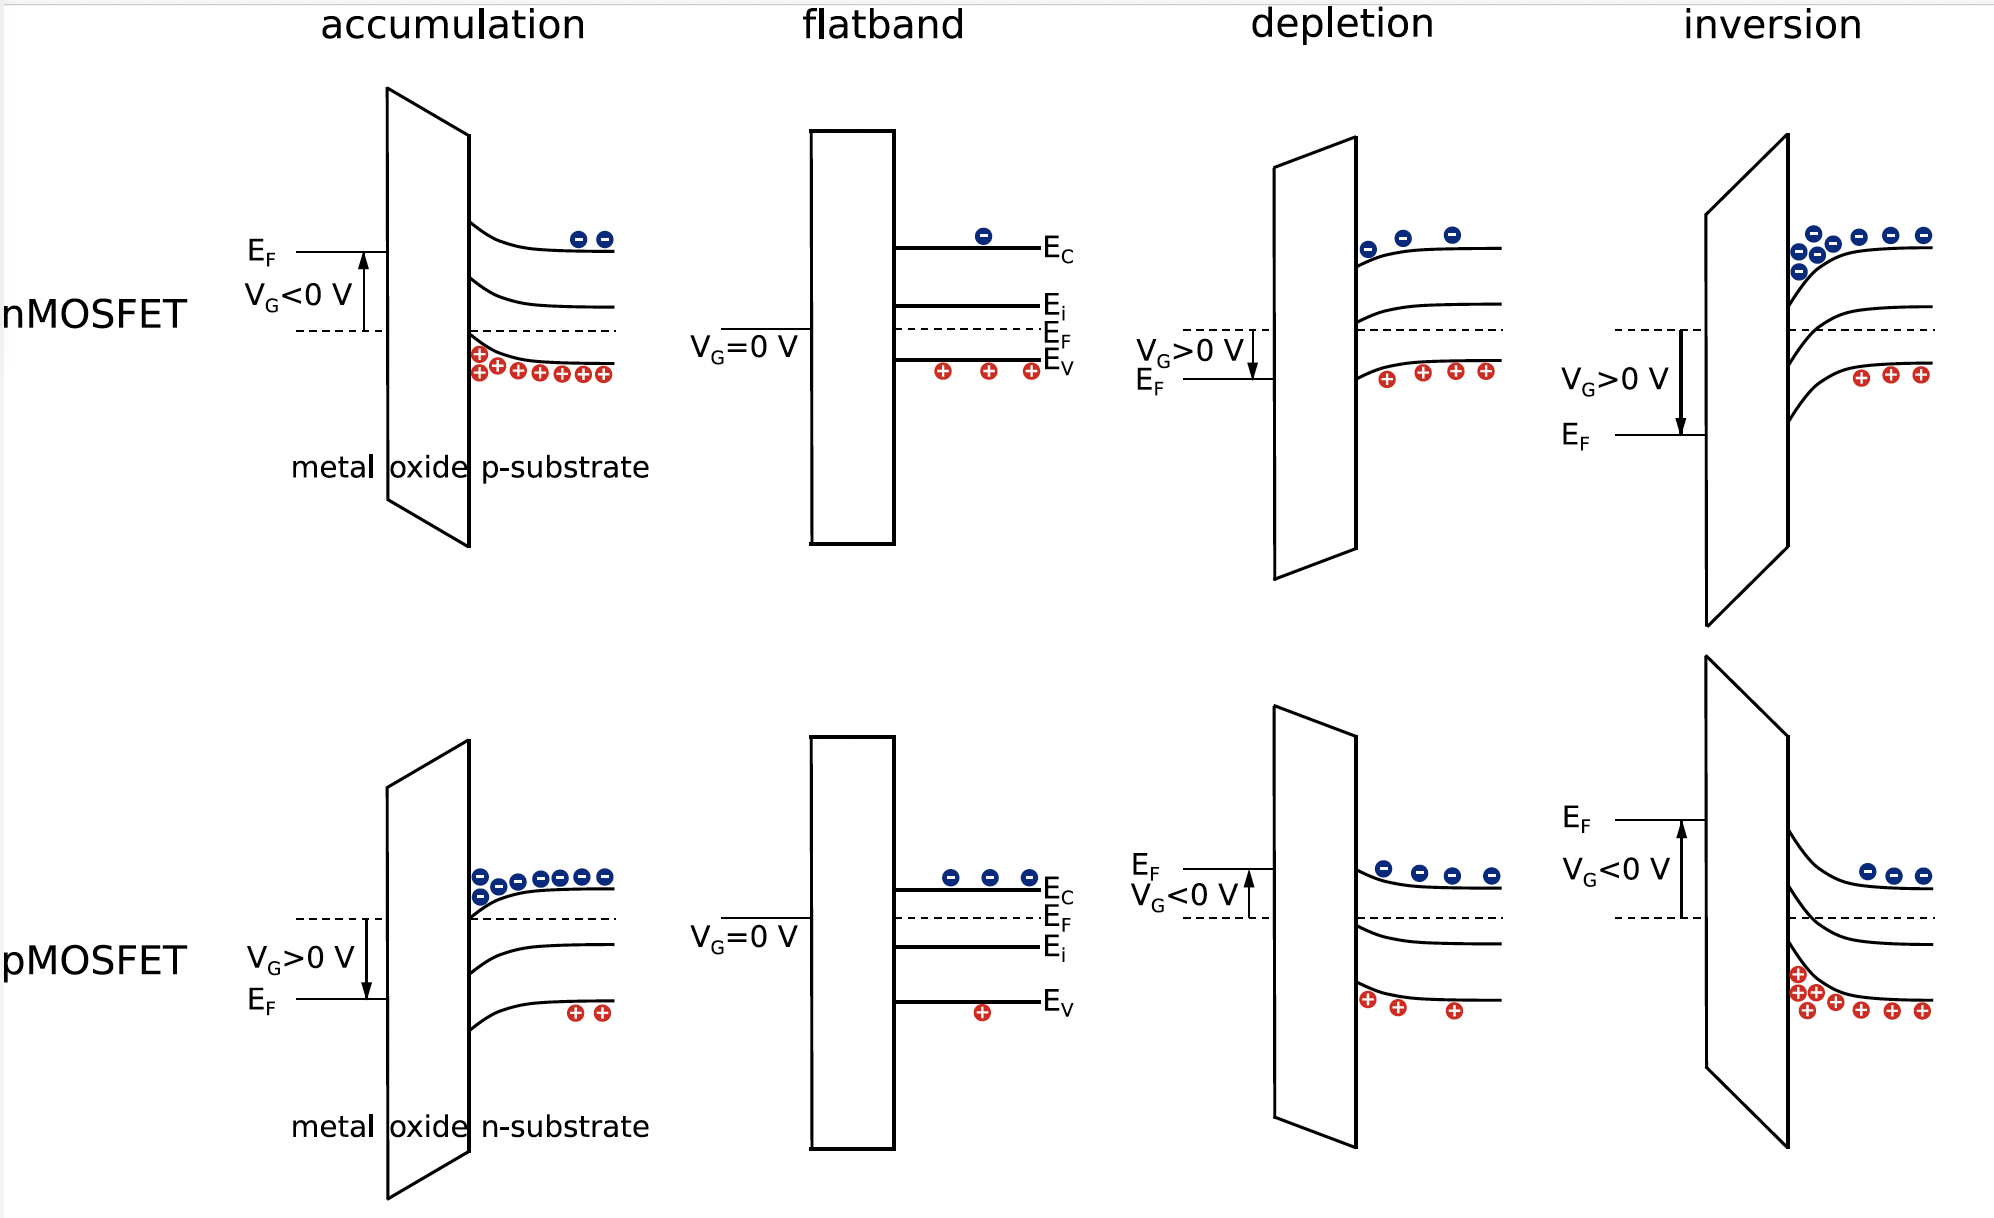
\includegraphics[width=5.0in]{2018spring/figures/16a_e.png}}
        \caption{The energy band diagrams for an ideal MOSFET capacitor: Under different bias conditions the MOSFET can be driven from accumulation (left) to inversion (right). Top: n-channel MOSFET (nMOSFET) Bottom: pMOSFET. In the case of a pMOSFET, a positive gate voltage (\( V_\mathrm {G} \)) accumulates the majority carriers of the substrate, which are electrons, in a layer near the oxide/substrate interface. In the band diagram shown in Figure 1.2, this means that the conduction band (\( E_\mathrm {C} \)) bends down towards the Fermi level (\( E_\mathrm {F} \)). When sweeping \( V_\mathrm {G} \) towards zero, the MOSFET reaches its flatband condition for \( V_\mathrm {G} \) \( = \) 0 V (ideal capacitor, otherwise the contact voltage must be considered), where the majority and minority carriers are in thermal equilibrium. By applying a low negative \( V_\mathrm {G} \) the majority carriers are forced away from the interface and therefore a depletion layer near the interface forms, which results in a bending up of the bands and the intrinsic energy (\( E_\mathrm {i} \)) moves closer to \( E_\mathrm {F} \). With further increasing negative \( V_\mathrm {G} \), the depletion layer is populated by minority carriers until \( V_\mathrm {G} \) exceeds a certain threshold voltage (\( V_{\mathrm {th}} \)) and the concentration of minority carriers is high enough to form a thin inversion layer near the interface. In the band diagram the inversion mode can be explained by a crossing of \( E_\mathrm {i} \) and \( E_\mathrm {F} \) where the minority carriers exceed the majority carriers at the interface. In this context it has to be mentioned, that \( V_{\mathrm {th}} \) is defined as a microscopic parameter which indicates the transition to the inversion mode.}
        \label{fig:16a_e}
        \end{figure}

        \begin{figure}
        \centering\fbox{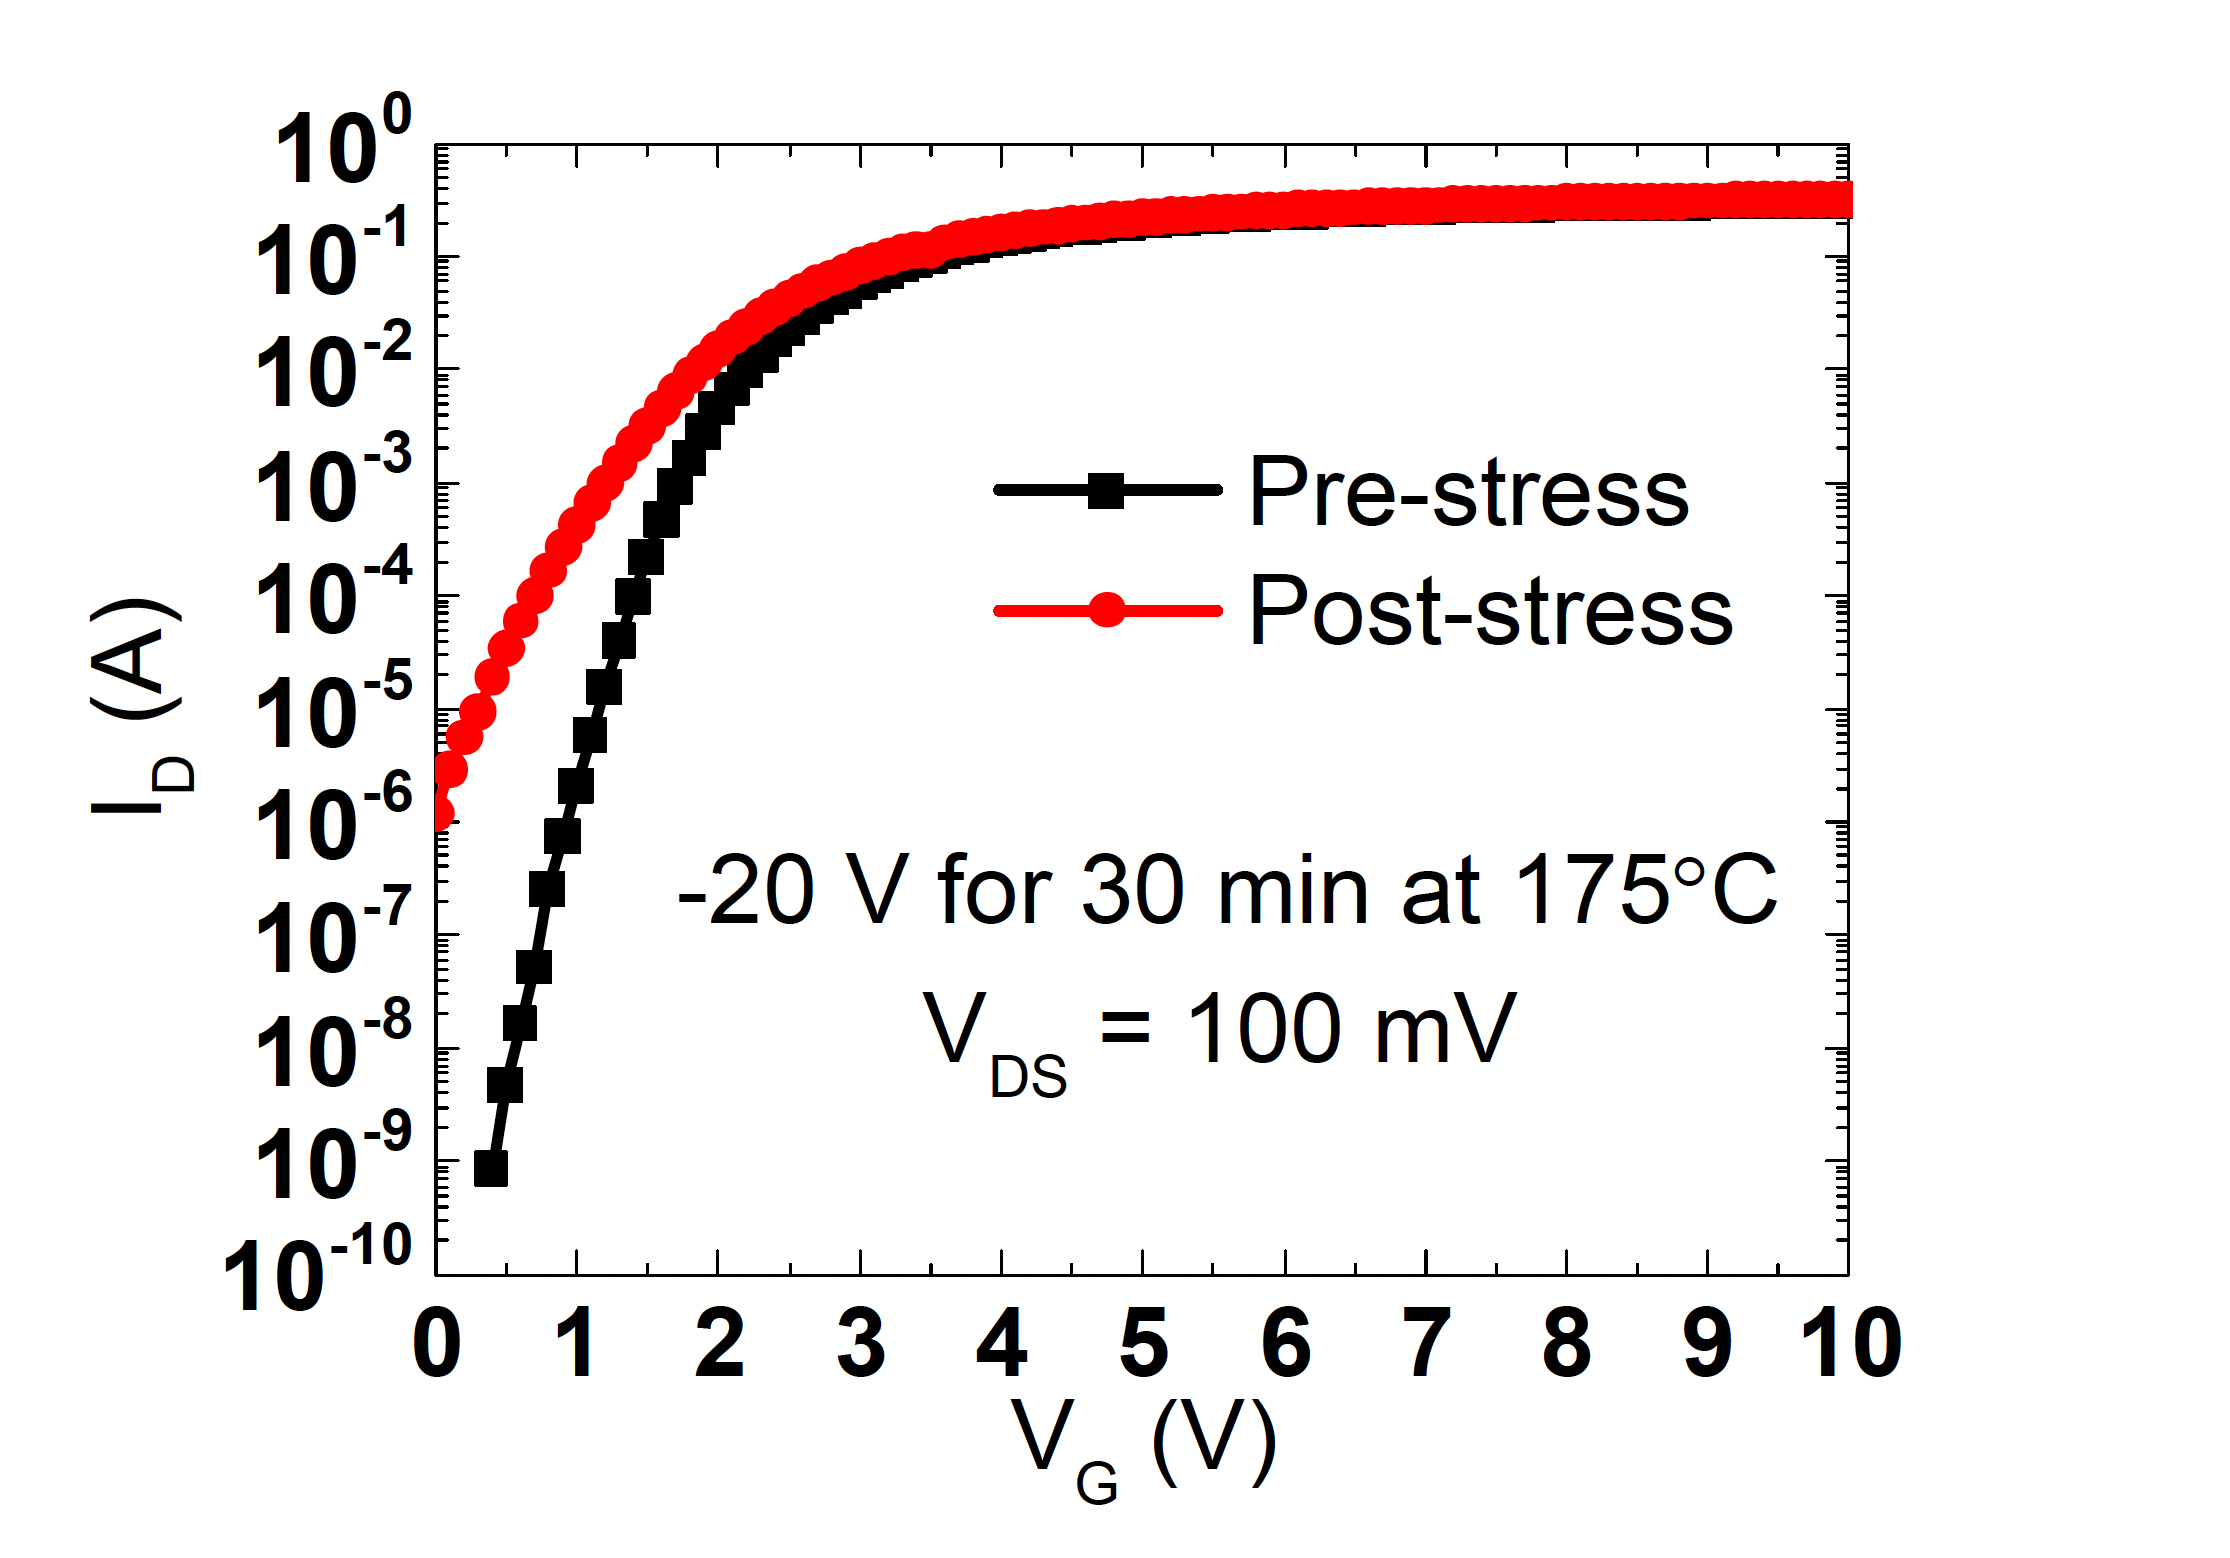
\includegraphics[width=3.0in]{2018spring/figures/16a_f.png}}
        \caption{$I_{D^{-}} V_G$ curves for a $1200 \mathrm{~V} \mathrm{SiC}$ power MOSFET taken at $175^{\circ} \mathrm{C}$ before and after a gate stress of $-20 \mathrm{~V}$ for thirty minutes.}
        \label{fig:16a_f}
        \end{figure}

    \end{enumerate}

\item [17.] MOS Capacitor

    \begin{figure}
    \centering\fbox{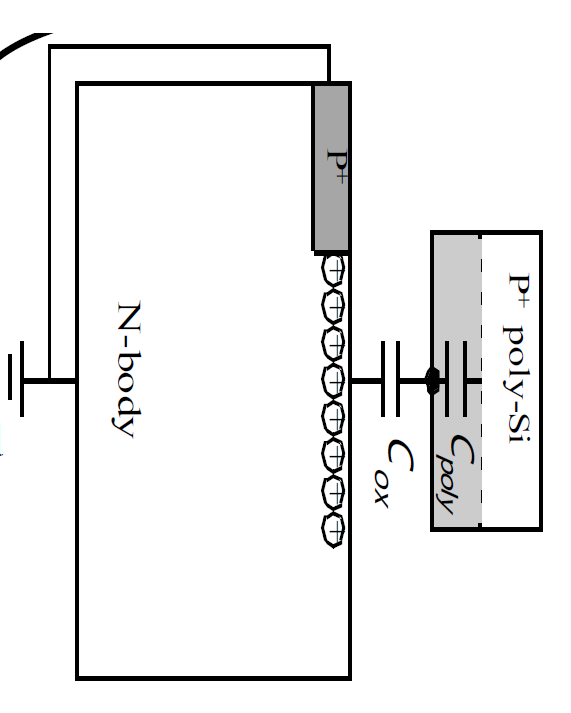
\includegraphics[width=3.0in]{2018spring/figures/17q_a.png}}
    \caption{Schematic of the poly depletion capacitance's upon gating this MOS capacitor. $\mathrm{T}=300\mathrm{K}$. Gate and body are Silicon. The gate oxide is \ch{SiO2}, $\mathrm{t}_{\mathrm{ox}} = 2 \mathrm{~nm}$ }
    \label{fig:17q_a}
    \end{figure}

    \begin{enumerate}
        \item \textbf{Q.} Draw the band diagram of a MOS system where the "metal" work function $\Phi_{\mathrm{M}}$ is larger than the silicon work function $\Phi_{\mathrm{S}}$. Assume that there are no applied voltages at the p-type substrate (doping $\mathrm{N}_{\mathrm{A}}$) and the gate. On the diagram clearly label the following parameters and functions: electron affinity in the semiconductor $\chi_{\mathrm{Sc}}$, the Fermi level $\mathrm{E}_{\mathrm{F}}$, the conduction and valance band edges $\mathrm{E}_{\mathrm{c}}$ and $\mathrm{E}_{\mathrm{V}}$, the band-gap $\mathrm{E}_{\mathrm{g}}$, the mid-gap $\mathrm{E}_{i}$, the thickness of the oxide $\mathrm{t}_{\mathrm{ox}}$, the potential drop in the oxide $\phi_{\mathrm{ox}}$, and the potential drop in the semiconductor $\phi(\mathrm{x})$. 
        
        \textbf{Theory} Reference figure \ref{fig:17t_a} and recall that the potential difference between conduction band and free space is called electron affinity and is denoted by $\chi_{\mathrm{Sc}}$. $E_0$ or $E_{vac}$ is the vacuum energy level where the electron is free from the material.

        \begin{figure}
        \centering\fbox{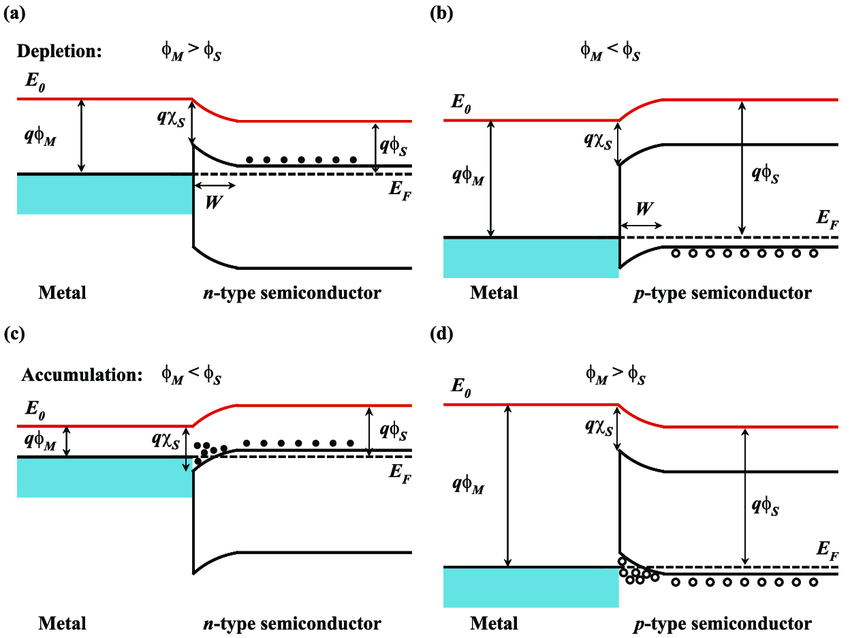
\includegraphics[width=5.0in]{2018spring/figures/17t_a.png}}
        \caption{Energy-band diagrams of metal-n-[(a) and (c)] or p-[(b) and (d)] type semiconductor contacts. Depending on the difference between work functions of the metal qφ M and of the semiconductor qφ S , the band bending results in either a depletion [(a) and (b)] or an accumulation [(c) and (d)] of charges at the metal-semiconductor interface.}
        \label{fig:17t_a}
        \end{figure}
        
        \textbf{A.} Shown in figure \ref{fig:17a_a} 

        \begin{figure}
        \centering\fbox{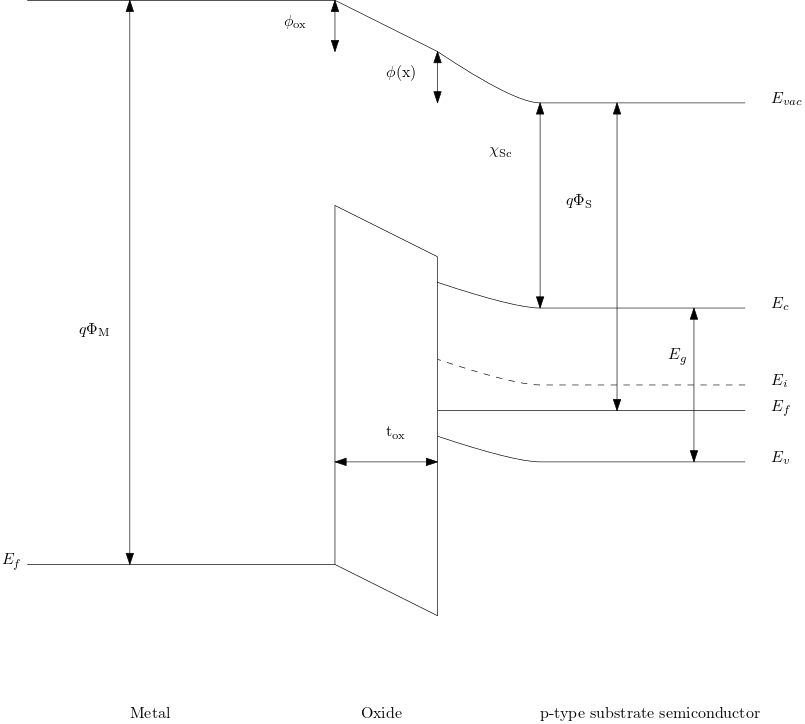
\includegraphics[width=5.0in]{2018spring/figures/17a_a.png}}
        \caption{MOS system where the "metal" work function $\Phi_{\mathrm{M}}$ is larger than the silicon work function $\Phi_{\mathrm{S}}$. No applied voltages at the p-type substrate (doping $\mathrm{N}_{\mathrm{A}}$) and the gate. Electron affinity in the semiconductor $\chi_{\mathrm{Sc}}$, Fermi level $\mathrm{E}_{\mathrm{F}}$, conduction and valance band edges $\mathrm{E}_{\mathrm{c}}$ and $\mathrm{E}_{\mathrm{V}}$, band-gap $\mathrm{E}_{\mathrm{g}}$, mid-gap $\mathrm{E}_{i}$, thickness of oxide $\mathrm{t}_{\mathrm{ox}}$, potential drop in the oxide $\phi_{\mathrm{ox}}$, and potential drop in the semiconductor $\phi(\mathrm{x})$.}
        \label{fig:17a_a}
        \end{figure}
        
        \item \textbf{Q.} For this device, what is the most likely outcome when no voltages are applied: inversion or accumulation? Why? \textbf{A.} Referencing figure \ref{fig:17t_a}, accumulation is more likely because $\Phi_{\mathrm{M}} > \Phi_{\mathrm{S}}$ and because the MOS has a p-type substrate.
        
        \item \textbf{Q.} Poly-Silicon Gate Depletion (refer to Figure \ref{fig:17q_a}): Assume the voltage $\mathrm{V}_{\mathrm{ox}} = \qty{1}{\volt}$ across a $\qty{2}{\nano\meter}$ thin \ch{SiO2} oxide. The $\mathrm{P}^{+}$ poly gate doping is $\mathrm{N}_{\text {poly }}=1 \times 10^{19} \mathrm{~cm}^{-3}$ and the substrate is n-doped with $\mathrm{N}_{\mathrm{D}}=10^{17} \mathrm{~cm}^{-3}$. Find the poly depletion width, $\mathrm{W}_{\mathrm{dep }}$. \textbf{Theory} A heavily doped film of polycrystalline silicon (poly-Si) is typically employed as the gate-electrode material in modern MOS devices. Refer to figure \ref{fig:17q_b}, and figure \ref{fig:17ac_b}. There are practical limits to the electrically active dopant concentration (usually less than $1 \times 10^{20} \mathrm{~cm}^{-3}$). The gate must be considered as a semiconductor, rather than a metal. 
      
        $$
        W_{poly}=\sqrt{\frac{2 \varepsilon_{Si} V_{poly}}{q N_{poly}}}
        $$

        \begin{figure}
        \centering\fbox{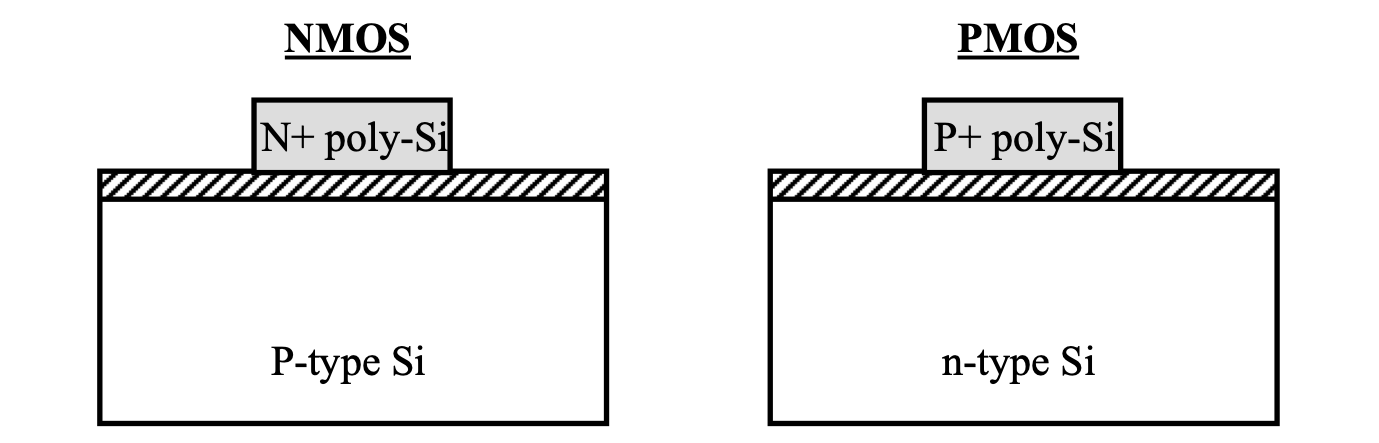
\includegraphics[width=5.0in]{2018spring/figures/17q_b.png}}
        \caption{Heavily doped film of polycrystalline silicon (poly-Si)}
        \label{fig:17q_b}
        \end{figure}

        \begin{figure}
        \centering\fbox{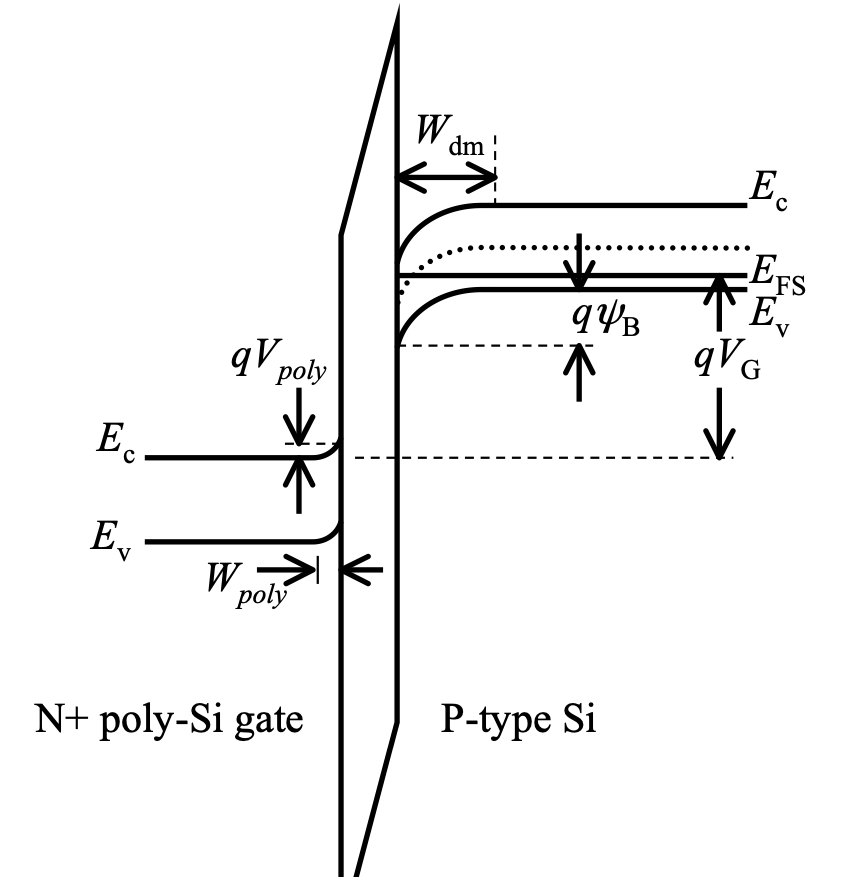
\includegraphics[width=5.0in]{2018spring/figures/17ac_b.png}}
        \caption{Si biased to inversion}
        \label{fig:17ac_b}
        \end{figure}
        
        \textbf{A.} The elementary charge, usually denoted by $e = 1.602176634 \times 10^{-19} \mathrm{C}$, $q$ in this problem, is the electric charge carried by a single proton or, equivalently, the magnitude of the negative electric charge carried by a single electron, which has charge $-1 e$. The $\mathrm{p}^{+}$ poly gate doping is $\mathrm{N}_{\text {poly }}=1 \times 10^{19} \mathrm{~cm}^{-3}$. The voltage $\mathrm{V}_{\mathrm{ox}} = \qty{1}{\volt}$ is across a $t_{ox} = \qty{2}{\nano\meter}$ thin \ch{SiO2} oxide. Vacuum permittivity, commonly denoted $\varepsilon_0$ (pronounced "epsilon nought" or "epsilon zero"), is the value of the absolute dielectric permittivity of classical vacuum. It may also be referred to as the permittivity of free space, the electric constant, or the distributed capacitance of the vacuum. It is an ideal (baseline) physical constant. Its CODATA value is: $\varepsilon_0=8.8541878128(13) \times 10^{-12} \mathrm{~F} \cdot \mathrm{m}^{-1}$ (farads per meter), with a relative uncertainty of $1.5 \times 10^{-10}$. The silicon dioxide $\mathrm{SiO}_2$ relative dielectric constant is 3.9. Gauss's Law dictates $W_{poly}=\varepsilon_{ox} {\varepsilon_{ox}} / q N_{poly}$.

        $$
        \begin{aligned}
        W_{poly} &= \frac{\varepsilon_{ox} \varepsilon_{ox}}{q N_{poly}}\\
        &= \frac{\varepsilon_{ox} V_{ox}}{t_{ox} q N_{poly}} \\
        &= \frac{3.9 \times 8.85 \times 10^{-14}(\mathrm{~F} / \mathrm{cm}) \cdot 1 \mathrm{~V}}{2 \times 10^{-7} \mathrm{~cm} \cdot 1.6 \times 10^{-19} \mathrm{C} \cdot 8 \times 10^{19} \mathrm{~cm}^{-3}} \\
        & =1.3 \mathrm{~nm}
        \end{aligned}
        $$
        
    \end{enumerate}
    


\item [18.] Basic \textit{pn}-junction operation.\\

Consider the ideal so-called "long-base" abrupt \textit{pn}-junction silicon diode that has a uniform cross section and constant doping on both sides of the \textit{pn}-junction. The diode is doped as follows: $\mathrm{N}_{\mathrm{a}}=8.0 \times 10^{16} \mathrm{~cm}^{-3}$ \textit{p}-type and $\mathrm{N}_{\mathrm{d}}=1 \mathrm{x} 10^{16} \mathrm{~cm}^{-3}$ \textit{n}-type. For this material, the minority-carrier lifetimes are: $\tau_{\mathrm{n}}=4 \times 10^{-6} \mathrm{~s}$ and $\tau_{\mathrm{p}}=1 \times 10^{-6} \mathrm{~s}$, respectively. You may assume that the effects within the space-charge region are negligible and that the minority carriers flow only by diffusion in the charge neutral regions.

    \begin{enumerate}
        \item \textbf{Q.} Draw/sketch the band-diagram for this system. Also, plot the electrostatic potential, the net charge density and the corresponding electric field. \textbf{A.} Figure \ref{fig:18a_a}.

        \begin{figure}
        \centering\fbox{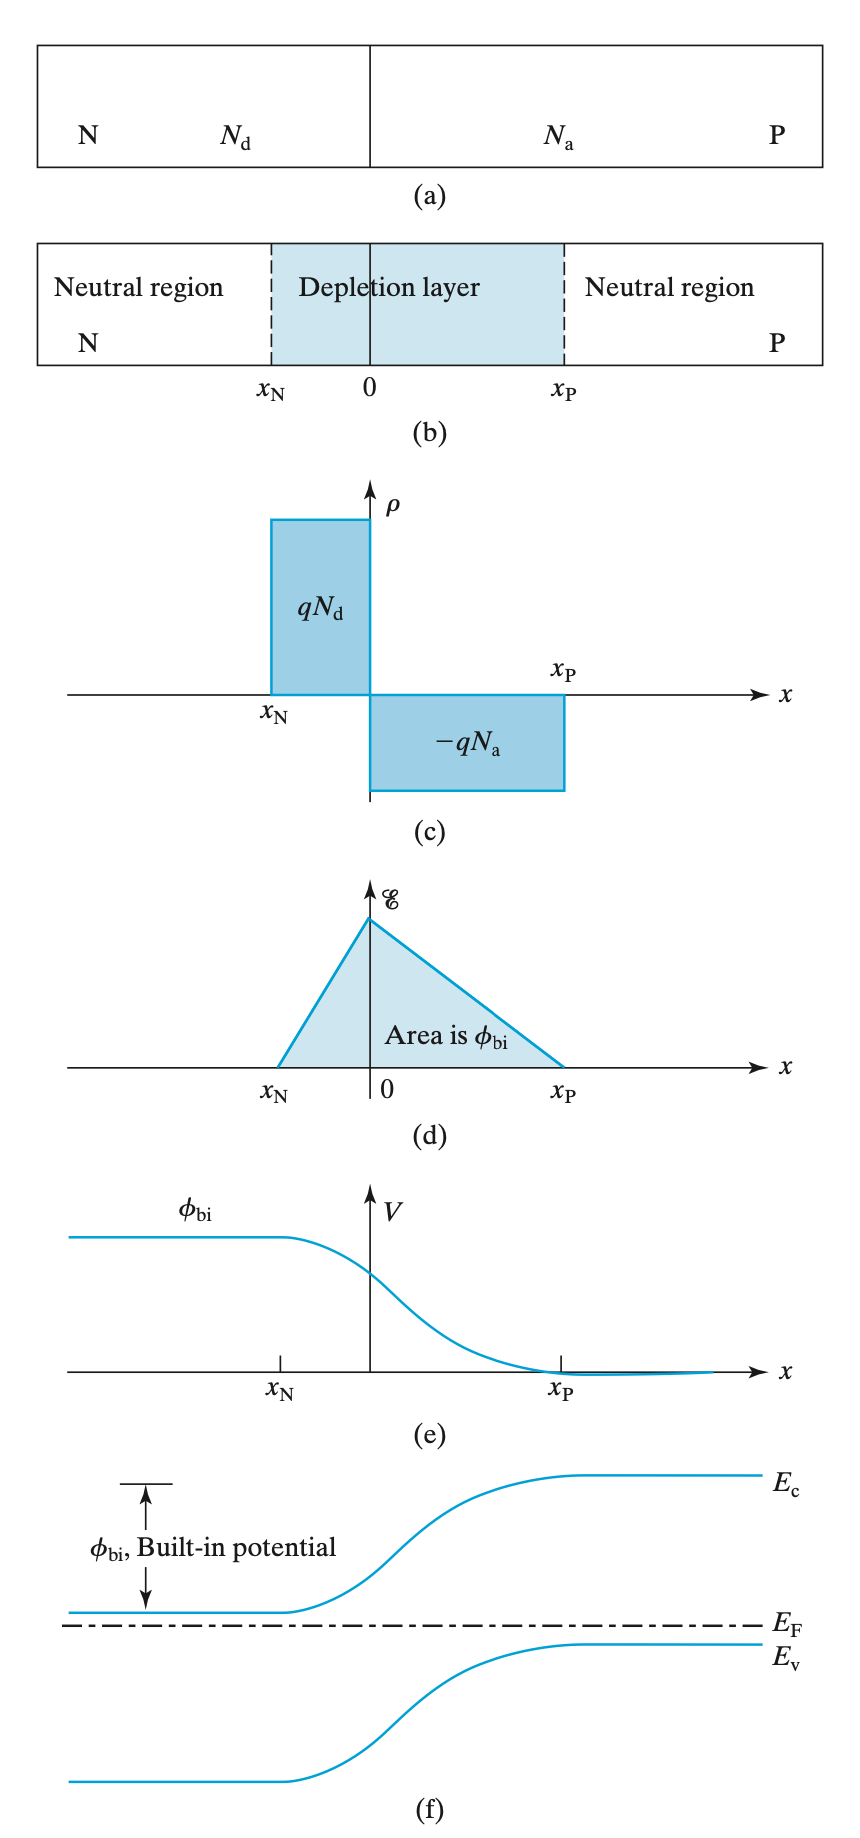
\includegraphics[width=3.0in]{2018spring/figures/18a_a.png}}
        \caption{Ideal so-called "long-base" abrupt \textit{pn}-junction band diagram. (a) Step PN junction; (b) depletion approximation; (c) space charge profile; (d) electric field from integration of $\rho / \varepsilon_s$ (Poisson's equation); (e) electric potential from integrating $-\mathscr{E}$; and (f) energy band diagram.}
        \label{fig:18a_a}
        \end{figure}
        
        \item \textbf{Q.} Determine the value of the built-in potential across the \textit{pn}-junction. \textbf{A.} The built-in potential across the pn junction can be determined using the formula:
        
        $$
        V_{b i}=\frac{k T}{q} \ln \left(\frac{N_a N_d}{n_i^2}\right)
        $$
        
        where $k$ is the Boltzmann constant, $T$ is the temperature in Kelvin, $q$ is the elementary charge, $N_a$ and $N_d$ are the acceptor and donor concentrations respectively, and $n_i$ is the intrinsic carrier concentration. For silicon at room temperature, $n_i$ is approximately $1.45 \times 10^{10} \mathrm{~cm}^{-3}$. Substituting the given values into the formula, we get:
        
        $$
        V_{b i}=\frac{k T}{q} \ln \left(\frac{8.0 \times 10^{16} \mathrm{~cm}^{-3} \times 1.0 \times 10^{16} \mathrm{~cm}}{\left(1.45 \times 10^{10} \mathrm{~cm}^{-3}\right)^2}\right).
        $$

        At room temperature $(T=300 K)$, this simplifies to:
        
        $$
        V_{b i}=0.0259 \mathrm{~V} \times \ln \left(3.01 \times 10^{24}\right)=0.74 \mathrm{~V}
        $$
        
        So, the built-in potential across the pnjunction is approximately $0.74 \mathrm{~V}$.
        
        \item \textbf{Q.} Calculate the density of the minority carriers at the edge of the space-charge region for a forward bias of 0.3V. \textbf{A.} The density of minority carriers at the edge of the space-charge region for a forward bias voltage $V$ can be calculated using the formula:
        
        $$
        n_p=n_{p 0} e^{q V / k T}
        $$
        
        for the $\mathrm{p}$-side, and
        
        $$
        p_n=p_{n 0} e^{q V / k T}
        $$
        
        for the $\mathrm{n}$-side, where
        
        $$
        n_{p 0}
        $$
        
        and $p_{n 0}$ are the equilibrium minority carrier concentrations on the $\mathrm{p}$-side and $\mathrm{n}$-side respectively, $q$ is the elementary charge, $k$ is the Boltzmann constant, and $T$ is the temperature in Kelvin. The equilibrium minority carrier concentrations can be calculated using the formula:
        
        $$
        n_{p 0}=\frac{n_i^2}{N_a}
        $$
        
        for the $\mathrm{p}$-side, and
        
        $$
        p_{n 0}=\frac{n_i^2}{N_d}
        $$
        
        for the $\mathrm{n}$-side, where $N_a$ and $N_d$ are the acceptor and donor concentrations respectively, and $n_i$ is the intrinsic carrier concentration. Substituting the given values into these formulas, we get:
        
        $$
        n_{p 0}=\frac{\left(1.45 \times 10^{10} \mathrm{~cm}^{-3}\right)^2}{8.0 \times 10^{16} \mathrm{~cm}^{-3}}=2.6 \times 10^3 \mathrm{~cm}^{-3}
        $$
        
        and
        
        $$
        p_{n 0}=\frac{\left(1.45 \times 10^{10} \mathrm{~cm}^{-3}\right)^2}{1.0 \times 10^{16} \mathrm{~cm}^{-3}}=2.1 \times 10^4 \mathrm{~cm}^{-3}
        $$
        
        For a forward bias of $0.3 \mathrm{~V}$, we get:
        
        $$
        n_p=\left(2.6 \times 10^3 \mathrm{~cm}^{-3}\right) e^{(0.3 V)\left(1.6 \times 10^{-19} \mathrm{C}\right) /\left(1.38 \times 10^{-23} J\right)}
        $$
        
        and
        
        $$
        p_n=\left(2.1 \times 10^4 \mathrm{~cm}^{-3}\right) e^{(0.3 V)\left(1.6 \times 10^{-19} \mathrm{C}\right) /\left(1.38 \times 10^{-23} J\right)}
        $$
        
        So, at a forward bias of $0.3 \mathrm{~V}$, the density of minority carriers at the edge of the space-charge region is approximately $7.5 \times 10^{4}$ $\mathrm{cm}^{-3}$ on the $p$-side and $6.1 \times 10^{5} \mathrm{~cm}^{-3}$ on the n-side.
        
        \item \textbf{Q.} Under bias condition, calculate and plot the minority and majority carrier currents as a function of distance from the junction. \textbf{A.} Steps for solving pn junction problems under bias.
        
        \begin{itemize}
            \item[1.] Solve minority carrier diffusion equations using the boundary conditions at the edge of the depletion region and contacts to obtain the decay of the minority carrier concentrations.
            \item[2.] Compute the minority carrier current densities in the quasi-neutral regions.
            \item[3.] Find the solutions for the currents at the edges of the depletion region and add the current densities at each edge of the depletion region.
        \end{itemize}
        
        Start with holes on the quasi-neutral n-region. To simplify the math, shift the origin to the 
        
        $$
        \quad 0=D_{\mathrm{P}} \frac{d^2 \Delta p_{\mathrm{n}}}{d x^{\prime 2}}-\frac{\Delta p_{\mathrm{n}}}{\tau_{\mathrm{p}}}
        $$ 
        
        n-edge: $x^{\prime} \geq 0$ shown in Figure \ref{fig:18ad_a}. Then apply boundary conditions: 

        \begin{figure}
        \centering\fbox{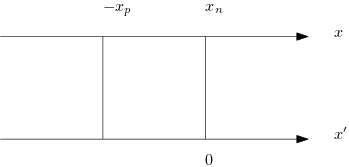
\includegraphics[width=2.0in]{2018spring/figures/18ad_a.png}}
        \caption{Shift origin to N edge}
        \label{fig:18ad_a}
        \end{figure}

        $$
        \begin{aligned}
        & \Delta p_{\mathrm{n}}\left(x^{\prime} \rightarrow \infty\right)=0 \\
        & \Delta p_{\mathrm{n}}\left(x^{\prime}=0\right)=\frac{n_{\mathrm{i}}^2}{N_{\mathrm{D}}}\left(e^{q v_{\mathrm{A}} / k T}-1\right)
        \end{aligned}
        $$

        From our previous discussions about the solution to the diffusion equation, we already know the general form of the solution

        $$
        \begin{aligned}
        \Delta p_{\mathrm{n}}\left(x^{\prime}\right) &= A_1 e^{-x^{\prime} / L_{\mathrm{P}}}+A_2 e^{x^{\prime} / L_{\mathrm{P}}} \\
        L_{\mathrm{P}} &= \sqrt{D_{\mathrm{P}} \tau_{\mathrm{p}}} \\
        A_1 &= \Delta p_n\left(x^{\prime}=0\right)
        \end{aligned}
        $$

        We can simplify by getting rid of $A_2$

        $$
        \begin{aligned}
        \Delta p_{\mathrm{n}}\left(x^{\prime}\right) &= \frac{n_{\mathrm{i}}^2}{N_{\mathrm{D}}}\left(e^{q V_{\mathrm{A}} / k T}-1\right) e^{-x^{\prime} / L_{\mathrm{P}}} \\
        J_{\mathrm{P}}\left(x^{\prime}\right) &= -q D_{\mathrm{P}} \frac{d \Delta p_{\mathrm{n}}}{d x^{\prime}}\\
        &= q \frac{D_{\mathrm{P}}}{L_{\mathrm{P}}} \frac{n_{\mathrm{P}}^2}{N_{\mathrm{D}}}\left(e^{q V_{\mathrm{A}} / k T}-1\right) e^{-x^{\prime} / L_{\mathrm{P}}}
        \end{aligned}
        $$

        Now shift the origin again and deal with the p-side of the junction shown in figure \ref{fig:18ad_b} and we get the same forms of the equations for the minority carrier concentrations and the current density:

        \begin{figure}
        \centering\fbox{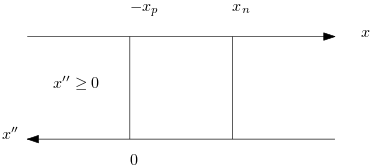
\includegraphics[width=2.0in]{2018spring/figures/18ad_b.png}}
        \caption{Shift origin to P edge}
        \label{fig:18ad_b}
        \end{figure}

        $$
        \begin{aligned}
        \Delta n_{\mathrm{p}}\left(x^{\prime \prime}\right) &= \frac{n_{\mathrm{i}}^2}{N_{\mathrm{A}}}\left(e^{q V_{\mathrm{A}} / k T}-1\right) e^{-x^7 / L_{\mathrm{N}}}\\
        J_{\mathrm{N}}\left(x^{\prime \prime}\right) &= -q D_{\mathrm{N}} \frac{d \Delta n_{\mathrm{P}}}{d x^{\prime \prime}}\\
        &= q \frac{D_{\mathrm{N}}}{L_{\mathrm{N}}} \frac{n_{\mathrm{i}}^2}{N_{\mathrm{A}}}\left(e^{q V_{\mathrm{A}} / k T}-1\right) e^{-x^{\prime} / L_{\mathrm{N}}}
        \end{aligned}
        $$

        Now evaluate the current at the edges of the depletion region and sum the contributions:

        $$
        \begin{aligned}            
        J_{\mathrm{N}}\left(x=-x_{\mathrm{p}}\right) &= J_{\mathrm{N}}\left(x^{\prime \prime}=0\right)\\
        &=q \frac{D_{\mathrm{N}}}{L_{\mathrm{N}}} \frac{n_i^2}{N_{\mathrm{A}}}\left(e^{q V_{\mathrm{A}} / k T}-1\right) \text{\quad electrons}\\
        J_{\mathrm{P}}\left(x=x_{\mathrm{n}}\right) &= J_{\mathrm{P}}\left(x^{\prime}=0\right)\\
        &=q \frac{D_{\mathrm{P}}}{L_{\mathrm{P}}} \frac{n_i^2}{N_{\mathrm{D}}}\left(e^{q V_{\mathrm{A}} / k T}-1\right) 
        \text{\quad holes}
        \end{aligned}
        $$

        Finally,

        $$
        \begin{aligned}
        I &=AJ \\
        &=qA\left(\frac{D_{\mathrm{N}}}{L_{\mathrm{N}}} \frac{n_{\mathrm{i}}^2}{N_{\mathrm{A}}}+\frac{D_{\mathrm{P}}}{L_{\mathrm{P}}} \frac{n_{\mathrm{i}}^2}{N_{\mathrm{D}}}\right)\left(e^{q V_{\mathrm{A}} / k T}-1\right)\\
        I &=I_0\left(e^{q V_{\mathrm{A}} / k T}-1\right) \\
        I_0 &\equiv q A\left(\frac{D_{\mathrm{N}}}{L_{\mathrm{N}}} \frac{n_{\mathrm{i}}^2}{N_{\mathrm{A}}}+\frac{D_{\mathrm{P}}}{L_{\mathrm{P}}} \frac{n_{\mathrm{i}}^2}{N_{\mathrm{D}}}\right)
        \end{aligned}
        $$

        So what happens to the carriers. We expect minority carrier concentrations on each side to vary with the applied bias. Due to the variations in the diffusion of carriers across the junction.

        $$
        \frac{p_p}{p_n}=e^{q V_0 / k T}
        $$

        Equilibrium hole concentrations on each side of the barrier. With bias this becomes: 

        $$
        \begin{aligned}
        \frac{p\left(-x_{p 0}\right)}{p\left(x_{n 0}\right)}=e^{q \left(V_0-V\right)/kT} \text{\quad altered barrier} 
        \end{aligned}
        $$

        Valid for forward and reverse bias. We assume low level injection - majority charge concentrations do not change. With low level injection, we can begin to simplify. The carrier concentrations are still changing despite the fact that we are neglecting the changes in the majority concentrations. Absolute increase of the majority concentrations means that there is an increase of the minimum concentrations $\left(p_p \text{ and } n_n\right)$ required to maintain charge neutrality. Relative changes in $p_p$ and $n_n$ vary only slightly compared to equilibrium values $p_0$ and $n_0$. Take the ratio of the concentrations with and without bias $\frac{p\left(x_{n 0}\right)}{p_n}=e^{q V / k T}$ assuming $p\left(-x_{p 0}\right)=p_p$. This equation gives us insight into the carrier concentration behavior under bias conditions. Under forward bias: the equation suggests a greatly increased hole concentration at the edge of the $n$ side. Conversely, the hole concentration under reverse bias is much smaller than the equilibrium value. Exponential increase in hole concentration at $x_{n0}$ with forward bias is an example of minority Quantitative PN Junction Current. We can determine the excess electrons and holes. Subtract the equilibrium concentrations.

        $$
        \frac{p_p}{p_n}=e^{q V_0 / k T}
        $$

        From the concentrations under bias.

        $$
        \begin{aligned}
        \frac{p\left(x_{n 0}\right)}{p_n} &= e^{q V / k T}\\
        \Delta p_n &= p\left(x_{n 0}\right)-p_n\\
        &= p_n\left(e^{q V / k T}-1\right)\\
        \Delta n_p &= n\left(-x_{p 0}\right)-n_p\prime\\
        &=n_p\left(e^{q V / k T}-1\right)
        \end{aligned}
        $$

        Should produce a distribution of excess holes in the $n$ material. As the holes diffuse, they recombine so the solution is identical to the diffusion equation. So we can write down the solution to the diffusion equation on either side of the junction. Excess electrons on p-side: 
        
        $$
        \delta n\left(x_p\right)=\Delta n_p e^{-x_p / L_n}=n_p\left(e^{q V / k T}-1\right) e^{-x_p / L_n}
        $$

        Excess holes on $n$-side:

        $$
        \delta p\left(x_n\right)=\Delta p_n e^{-x_n / L_p}=p_n\left(e^{q V / k T}-1\right) e^{-x_n / L_p}
        $$

        
        Now we understand the hole diffusion current at any point.

        $$
        I_p\left(x_n\right) &= -q A D_p \frac{d \delta p\left(x_n\right)}{d x_n}=q A \frac{D_p}{L_p} \Delta p_n e^{-x_n L_p}=q A \frac{D_p}{L_p} \delta p\left(x_n\right)
        $$

        Hole diffusion proportional to excess hole concentration. So what is the total current injected into the $n$-material?

        $$
        \begin{aligned}
        I_p\left(x_n=0\right) &= \frac{q A D_p}{L_p} \Delta p_n\\
        &=\frac{q A D_p}{L_p} p_n\left(e^{q V / k T}-1\right)\\
        I_n\left(x_p=0\right) &=-\frac{q A D_n}{L_n} \Delta n_p\\
        &=-\frac{q A D_n}{L_n} n_p\left(e^{q V / k T}-1\right)
        \end{aligned}
        $$

        Minus arises from current being directed opposite to $x_p$. Take $+x$ as the reference direction, what is the total current? The total current must be the sum of the electron and hole contributions.

        $$
        I=I_p\left(x_n=0\right)-I_n\left(x_p=0\right)=\frac{q A D_p}{L_p} \Delta p_n+\frac{q A D_n}{L_n} \Delta n_p
        $$

        Which can be simplified to the Diode Equation.

        $$
        I=q A\left(\frac{D_p}{L_p} p_n+\frac{D_n}{L_n} n_p\right)\left(e^{q V / k T}-1\right)=I_0\left(e^{q V / k T}-1\right)
        $$

        In arriving at this equation we have made no assumptions as to the sign of the bias voltage, and bias may be either forward or reverse. Let's check reverse bias $\left(V=-V_r\right)$. The total current then becomes: $I=q A\left(\frac{D_p}{L_p} p_n+\frac{D_n}{L_n} n_p\right)\left(e^{-q V_r / k T}-1\right)$. If $V_r$ is larger than a few $k T / q$: $I=-q A\left(\frac{D_p}{L_p} p_n+\frac{D_n}{L_n} n_p\right)=-I_0$. But what does the diode equation imply? The current is dominated by the injection of carriers from the more heavily doped side. We can, in most cases, simplify the diode equation to include only the contribution from the more heavily doped side. There are two ways to calculate current, slope of minority carrier concentrations (shown), and steady state charge storage. Reference figure \ref{fig:18ad_c}.

        \begin{figure}
        \centering\fbox{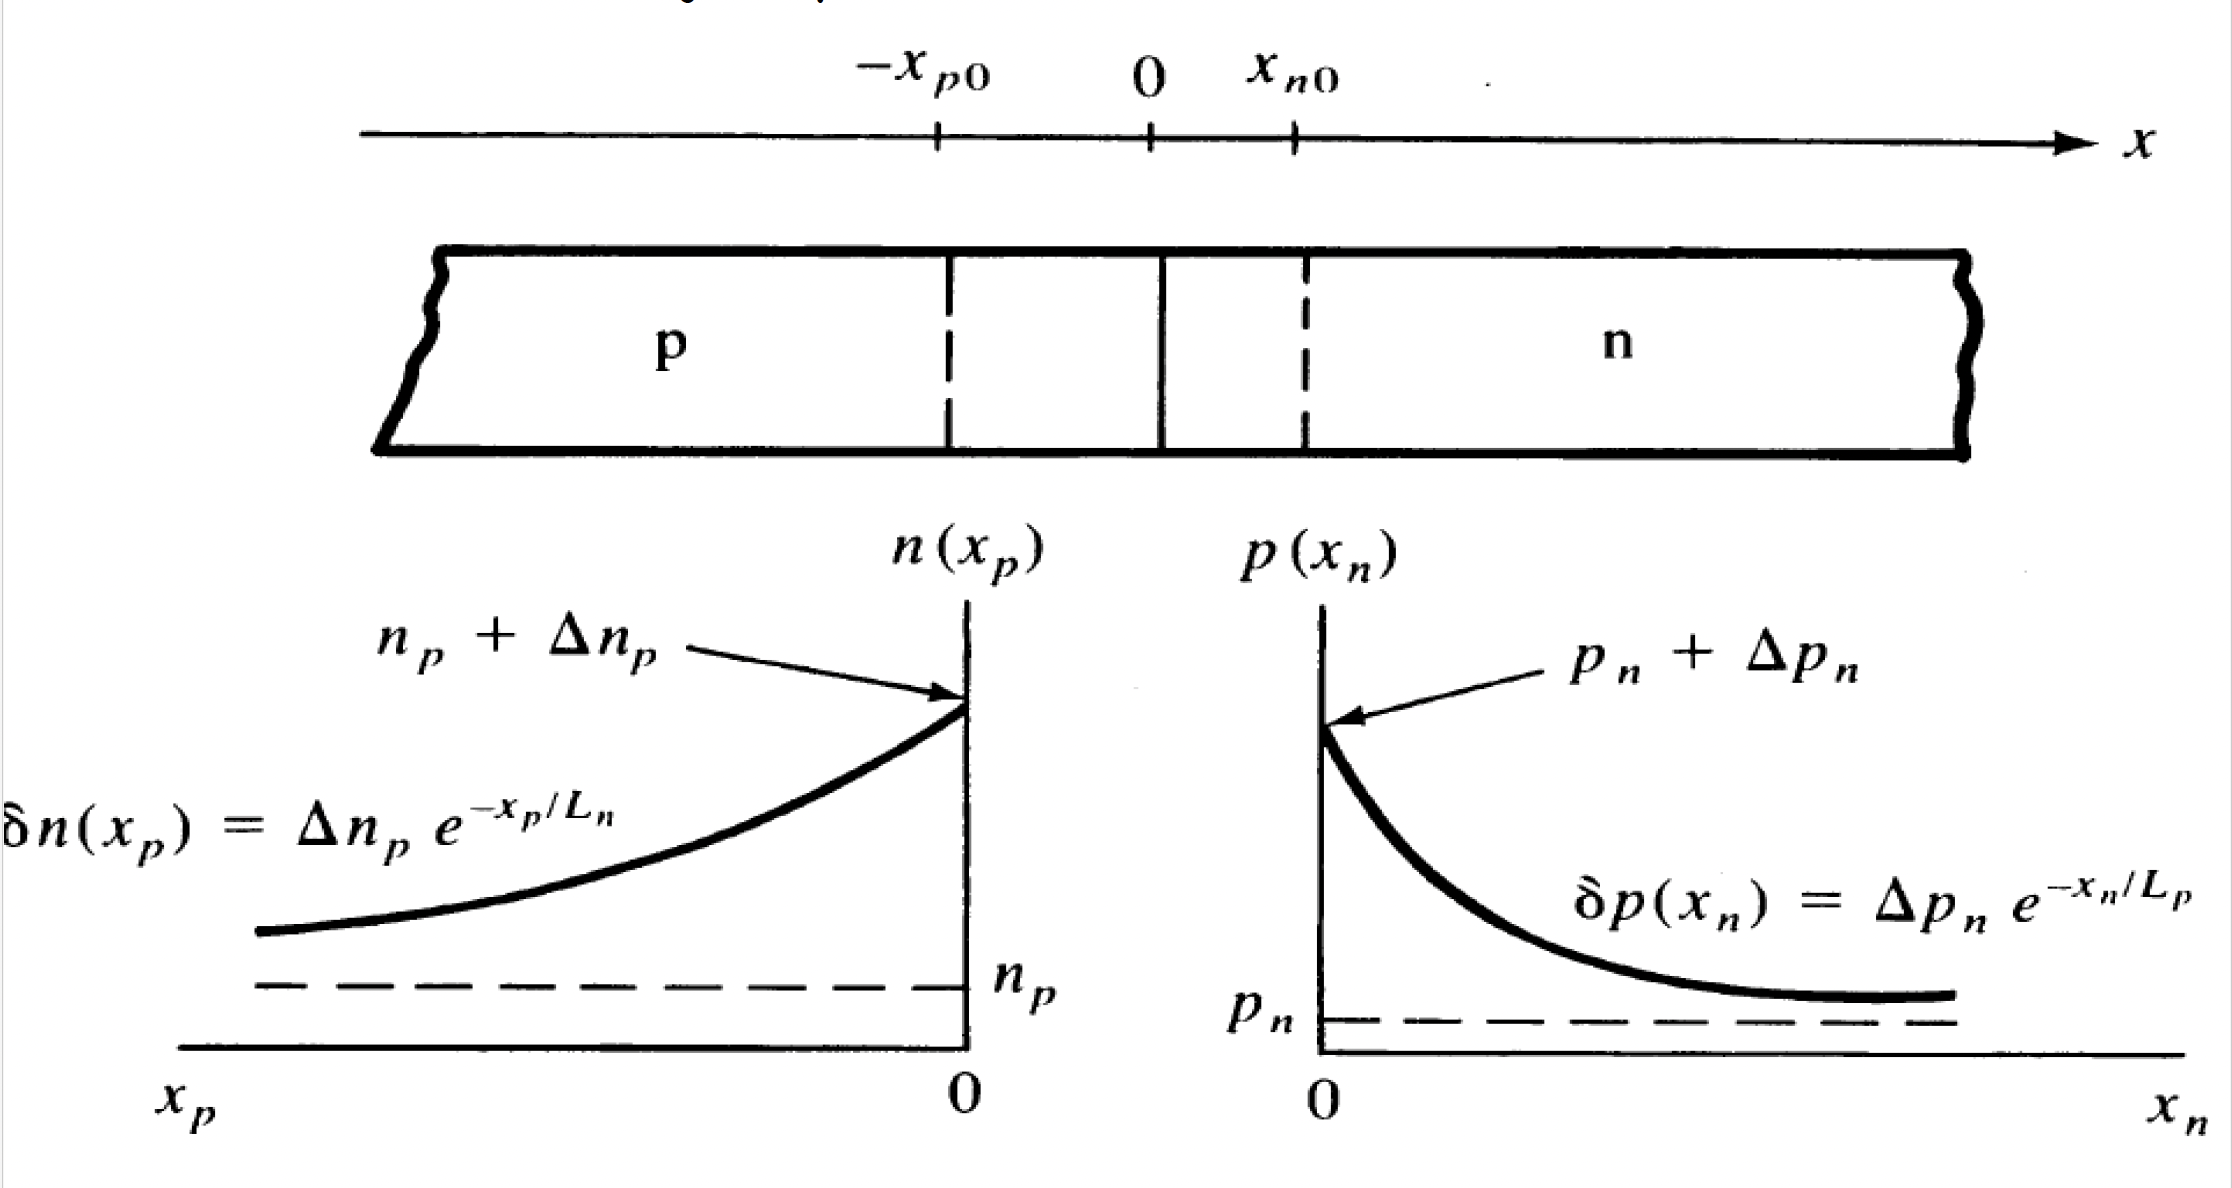
\includegraphics[width=5.0in]{2018spring/figures/18ad_c.png}}
        \caption{Minority and majority carrier currents as a function of distance from the junction}
        \label{fig:18ad_c}
        \end{figure}

    \end{enumerate}

\end{enumerate}
\end{document}